% !TEX encoding = UTF-8
% !TEX TS-program = pdflatex
% !TEX root = ../tesi.tex

%**************************************************************
\chapter{Analisi dei requisiti}
\label{cap:analisi-requisiti}
%**************************************************************

In questo capitolo vengono descritti i casi d'uso e i requisiti della piattaforma \textit{moviORDER}, individuati e classificati per definire nel dettaglio obiettivi e funzionalità del sistema. I casi d'uso e i requisiti sono stati dedotti da un'analisi preliminare eseguita dal \textit{tutor} aziendale, la quale è stata perfezionata dallo stagista per perseguire massima efficienza ed efficacia del sistema. Le convenzioni adottate per il codice univoco di casi d'uso e requisiti sono presentate in Appendice §\ref{convenzioni}.

\section{Casi d'uso}

La descrizione di ogni caso d'uso si compone dei seguenti punti:
\begin{enumerate}
	\item \textbf{attori}: lista di attori principali e secondari coinvolti nel caso d'uso;
    \item \textbf{descrizione}: breve descrizione del caso d'uso;
    \item \textbf{pre-condizioni}: condizioni che devono essere verificate prima dell'esecuzione del caso d'uso;
    \item \textbf{post-condizioni}: condizioni che devono essere verificate dopo dell'esecuzione del caso d'uso;
    \item \textbf{scenario principale}: descrizione composta dal flusso dei sottocasi del caso d'uso principale;
    \item \textbf{scenari alternativi}: descrizione composta dai casi d'uso che non appartengono al flusso
    principale di esecuzione del caso d'uso. Questo punto può essere omesso se non vi sono scenari alternativi;
    \item \textbf{specializzazioni}: indica quali sono tutte le specializzazioni del caso d'uso. Questo punto può essere omesso se non vi sono specializzazioni;
    \item \textbf{generalizzazioni}: indica quali sono tutte le generalizzazioni del caso d'uso. Questo punto può essere omesso se non vi sono generalizzaioni.
\end{enumerate}
Per lo studio dei casi di utilizzo più complessi della piattaforma sono stati creati dei diagrammi dei casi d'uso, che descrivono funzioni e/o servizi offerti dal sistema, così come sono percepiti e utilizzati dagli attori che interagiscono con lo stesso. Per la definizione dei diagrammi \textit{UML} dei casi d'uso è stato utilizzato lo standard \textit{UML 2.0}. 

\subsection{Attori del sistema}

Lo scopo di \textit{moviORDER} è fornire un'applicazione multipiattaforma per la vendita di prodotti. \textit{MoviORDER} viene distribuita da \visione{} alle aziende che forniscono prodotti, le quali la distribuiscono successivamente ai propri clienti. Gli utilizzatori finali di \textit{moviORDER} sono quindi gli utenti delle singole aziende clienti di \visione{}.
L'accesso all'applicazione è consentito solamente agli utenti provvisti di credenziali di accesso, le quali vengono distribuite insieme all'applicazione dal fornitore. Non è prevista quindi una funzionalità di registrazione. Nel contesto di \textit{moviORDER} vi sono per cui due tipologie di \glossaryItem{attori}:
\begin{enumerate}
	\item \textbf{Utente non autenticato}: è un utente che non ha effettuato l'accesso al sistema, al quale viene offerta la sola funzionalità di autenticazione. Una volta che un utente non autenticato accede al sistema, diventa un utente autenticato;
	\item \textbf{Utente autenticato}: è un utente che ha effettuato l'accesso al sistema e che può usufruire di tutte le sue funzionalità. All'utente autenticato è permesso di:
	\begin{itemize}
		\item effettuare il \textit{logout};
		\item aggiungere articoli al proprio carrello;
		\item modificare gli articoli nel proprio carrello;
		\item rimuovere articoli dal proprio carrello;
		\item inviare un ordine alla propria azienda.
	\end{itemize}
\end{enumerate}

\subsection{UC1 - Azioni utente non autenticato}

\begin{figure}[!h] 
    \centering 
    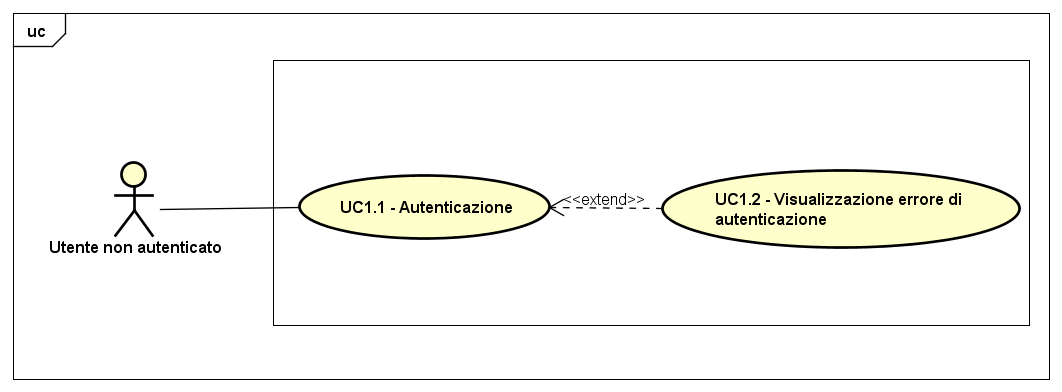
\includegraphics[width=\columnwidth]{usecase/generaleNonAutenticato} 
    \caption{\textit{Use Case} - UC1: Azioni utente non autenticato}
\end{figure}

\begin{itemize}
	\item \textbf{Attore}: Utente non autenticato;
	\item \textbf{Descrizione}: L'attore può eseguire l'operazione di autenticazione alla piattaforma \textit{moviORDER};
	\item \textbf{Pre-condizioni}: L'attore ha avviato l'applicazione e non è ancora stato riconosciuto dal sistema;
	\item \textbf{Post-condizioni}: L'attore ha eseguito l'operazione che desiderava compiere da utente non autenticato;
	\item \textbf{Scenario principale}: UC1.1 - Autenticazione;
	\item \textbf{Scenario alternativo}: L'attore ha fornito credenziali di accesso non corrispondenti a nessun utente registrato dall'azienda, oppure non riesce ad accedere al sistema perché è stato bloccato dall'azienda stessa: UC1.2 - Visualizzazione errore di autenticazione. 
\end{itemize}

\subsection{UC1.1 - Autenticazione}

\begin{figure}[!h] 
    \centering 
    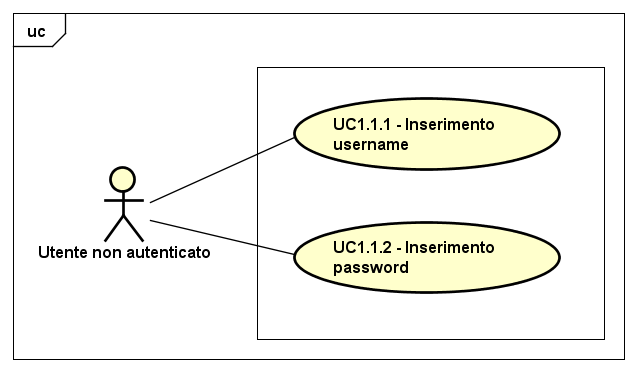
\includegraphics[width=\columnwidth]{usecase/autenticazione} 
    \caption{\textit{Use Case} - UC1.1: Autenticazione}
\end{figure}

\begin{itemize}
	\item \textbf{Attore}: Utente non autenticato;
	\item \textbf{Descrizione}: L'attore può eseguire l'operazione di autenticazione;
	\item \textbf{Pre-condizioni}: L'attore ha avviato l'applicazione, non è ancora riconosciuto dal sistema e ha espresso la volontà di effettuare l'autenticazione a \textit{moviORDER};
	\item \textbf{Post-condizioni}: L'attore ha eseguito l'operazione di accesso al sistema ed è quindi ora riconosciuto come utente autenticato;
	\item \textbf{Scenario principale}: 
		\begin{enumerate}
			\item UC1.1.1 - Inserimento \textit{username};
			\item UC1.1.2 - Inserimento \textit{password}.
		\end{enumerate} 
\end{itemize}

\subsection{UC1.1.1 - Inserimento \textit{username}}

\begin{itemize}
	\item \textbf{Attore}: Utente non autenticato;
	\item \textbf{Descrizione}: L'attore deve inserire una \textit{username} per l'operazione di autenticazione;
	\item \textbf{Pre-condizioni}: L'attore ha avviato l'applicazione, non è ancora riconosciuto dal sistema e il sistema richiede l'inserimento di una \textit{username} per l'operazione di autenticazione;
	\item \textbf{Post-condizioni}: L'attore ha inserito la \textit{username} per l'operazione di autenticazione;
	\item \textbf{Scenario principale}: L'attore inserisce la \textit{username} tramite una \textit{text box}.
\end{itemize}

\subsection{UC1.1.2 - Inserimento \textit{password}}

\begin{itemize}
	\item \textbf{Attore}: Utente non autenticato;
	\item \textbf{Descrizione}: L'attore deve inserire una \textit{password} per l'operazione di autenticazione;
	\item \textbf{Pre-condizioni}: L'attore ha avviato l'applicazione, non è ancora riconosciuto dal sistema e il sistema richiede l'inserimento di una \textit{password} per l'operazione di autenticazione;
	\item \textbf{Post-condizioni}: L'attore ha inserito la \textit{password} per l'operazione di autenticazione;
	\item \textbf{Scenario principale}: L'attore inserisce la \textit{password} tramite una \textit{text box}.
\end{itemize}

\subsection{UC1.2 - Visualizzazione errore di autenticazione}

\begin{itemize}
	\item \textbf{Attore}: Utente non autenticato;
	\item \textbf{Descrizione}: L'attore inserisce credenziali di accesso non corrispondenti a nessun utente registrato dall'azienda, oppure l'utente è stato bloccato dall'azienda stessa;
	\item \textbf{Pre-condizioni}: L'attore ha avviato l'applicazione, non è ancora riconosciuto dal sistema e inserisce credenziali di accesso non corrispondenti a nessun utente registrato dall'azienda, oppure è stato bloccato;
	\item \textbf{Post-condizioni}: L'attore ha visualizzato un messaggio d'errore relativo all'impossibilità di eseguire l'autenticazione per inserimento di credenziali errate o perché è stato bloccato;
	\item \textbf{Scenario principale}: L'attore visualizza un messaggio d'errore relativo all'impossibilità di eseguire l'autenticazione per inserimento di credenziali errate o perché è stato bloccato.
\end{itemize}

\newpage

\subsection{UC2 - Azioni utente autenticato}

\begin{figure}[!h] 
    \centering 
    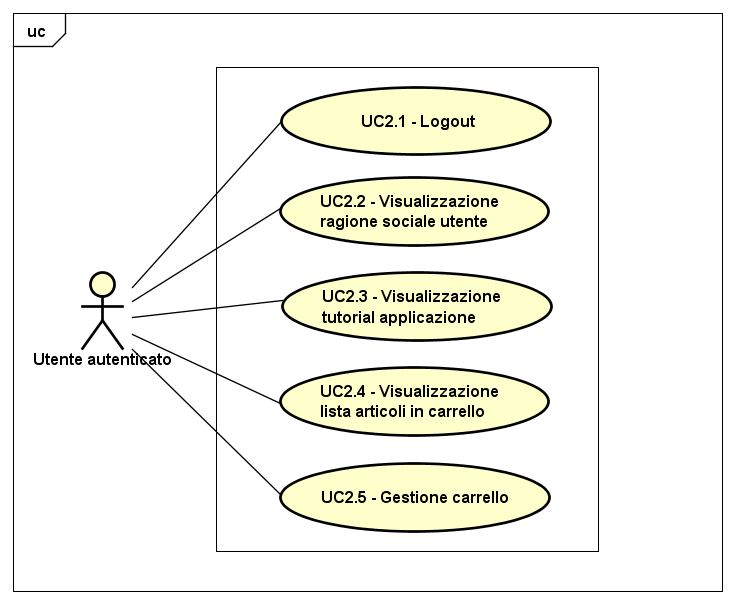
\includegraphics[width=\columnwidth]{usecase/generaleAutenticato} 
    \caption{\textit{Use Case} - UC2: Azioni utente autenticato}
\end{figure}

\begin{itemize}
	\item \textbf{Attore}: Utente autenticato;
	\item \textbf{Descrizione}: L'attore può:
	\begin{enumerate}
		\item eseguire l'operazione di \textit{logout};
		\item visualizzare il \textit{tutorial} dell'applicazione;
		\item gestire il proprio carrello. 
	\end{enumerate}
	\item \textbf{Pre-condizioni}: L'attore ha avviato l'applicazione ed è riconosciuto dal sistema;
	\item \textbf{Post-condizioni}: L'attore ha eseguito le azioni che desiderava compiere da utente autenticato;
	\item \textbf{Scenario principale}: 
		\begin{enumerate}
			\item UC2.1 - \textit{Logout};
			\item UC2.2 - Visualizzazione \textit{tutorial} applicazione;
			\item UC2.3 - Gestione carrello.
		\end{enumerate}
\end{itemize}

\subsection{UC2.1 - \textit{Logout}}

\begin{itemize}
	\item \textbf{Attore}: Utente autenticato;
	\item \textbf{Descrizione}: L'attore può eseguire l'operazione di \textit{logout};
	\item \textbf{Pre-condizioni}: L'attore ha avviato l'applicazione, è riconosciuto dal sistema e ha espresso la volontà di effettuare il \textit{logout} da \textit{moviORDER};
	\item \textbf{Post-condizioni}: L'attore ha eseguito l'operazione di \textit{logout} da \textit{moviORDER} ed è quindi uscito dal sistema tornando ad essere un utente non autenticato;
	\item \textbf{Scenario principale}: L'attore esegue l'operazione di \textit{logout} da \textit{moviORDER} premendo sul relativo bottone.
\end{itemize}

\subsection{UC2.2 - Visualizzazione \textit{tutorial} applicazione}

\begin{itemize}
	\item \textbf{Attore}: Utente autenticato;
	\item \textbf{Descrizione}: L'attore può visualizzare il \textit{tutorial} dell'applicazione;
	\item \textbf{Pre-condizioni}: L'attore ha avviato l'applicazione, è riconosciuto dal sistema e ha richiesto la visualizzazione del \textit{tutorial} dell'applicazione;
	\item \textbf{Post-condizioni}: L'attore ha visualizzato il \textit{tutorial} dell'applicazione;
	\item \textbf{Scenario principale}: L'attore visualizza il \textit{tutorial} dell'applicazione premendo sul relativo bottone.
\end{itemize}

\newpage

\subsection{UC2.3 - Gestione carrello}

\begin{figure}[!h] 
    \centering 
    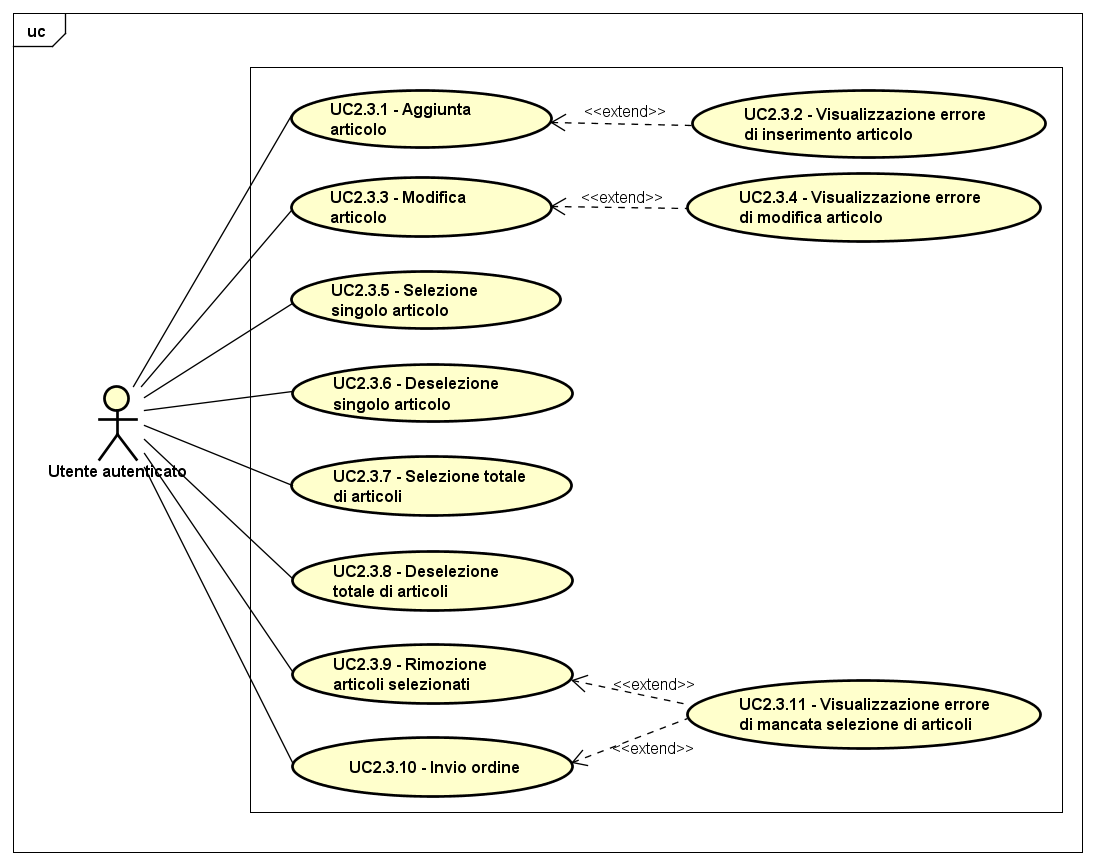
\includegraphics[width=\columnwidth]{usecase/gestioneCarrello} 
    \caption{\textit{Use Case} - UC2.3: Gestione carrello}
\end{figure}

\begin{itemize}
	\item \textbf{Attore}: Utente autenticato;
	\item \textbf{Descrizione}: L'attore può:
		\begin{enumerate}
			\item aggiungere un articolo al carrello;
			\item modificare un articolo in carrello;
			\item selezionare un singolo articolo in carrello;
			\item deselezionare un singolo articolo in carrello;
			\item selezionare tutti gli articoli in carrello;
			\item deselezionare tutti gli articoli in carrello;
			\item rimuovere articoli dal carrello;
			\item inviare un ordine.
		\end{enumerate}
	\item \textbf{Pre-condizioni}: L'attore ha avviato l'applicazione ed è riconosciuto dal sistema;
	\item \textbf{Post-condizioni}: L'attore ha eseguito le operazioni che desiderava compiere sul proprio carrello;
	\item \textbf{Scenario principale}:
		\begin{enumerate}
			\item UC2.3.1 - Aggiunta articolo;
			\item UC2.3.3 - Modifica articolo;
			\item UC2.3.5 - Selezione singolo articolo;
			\item UC2.3.6 - Deselezione singolo articolo;
			\item UC2.3.7 - Selezione totale di articoli;
			\item UC2.3.8 - Deselezione totale di articoli;
			\item UC2.3.9 - Rimozione articoli selezionati;
			\item UC2.3.10 - Invio ordine.
		\end{enumerate}
	\item \textbf{Scenari alternativi}:
		\begin{itemize}
			\item Durante l'operazione di aggiunta articolo, l'attore ha inserito un codice non corrispondente a nessun articolo venduto dall'azienda, oppure ha inserito una quantità non permessa per l'articolo, oppure la scansione del codice a barre per la ricerca del codice articolo è fallita: UC2.3.2 - Visualizzazione errore di inserimento articolo;
			\item Durante l'operazione di modifica articolo, l'attore ha inserito una quantità non permessa per l'articolo: UC2.3.4 - Visualizzazione errore di modifica articolo;
			\item L'attore ha premuto il bottone per la rimozione degli articoli selezionati senza aver selezionato alcun articolo dal carrello: UC2.3.11 - Visualizzazione errore di mancata selezione di articoli;
			\item L'attore ha premuto il invio di un ordine senza aver selezionato alcun articolo dal carrello: UC2.3.12 - Visualizzazione errore di mancata selezione di articoli.
		\end{itemize}
\end{itemize}

\newpage

\subsection{UC2.3.1 - Aggiunta articolo}

\begin{figure}[!h] 
    \centering 
    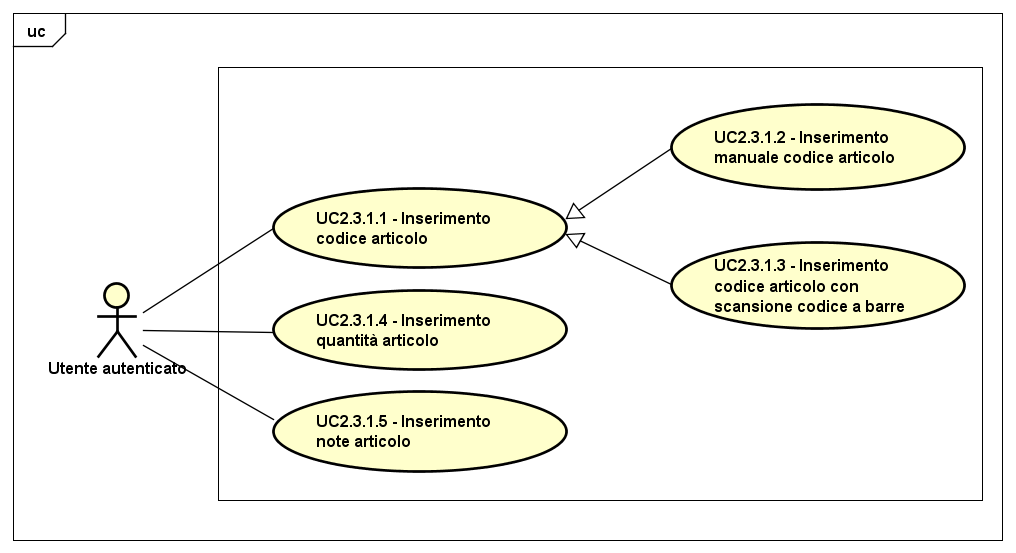
\includegraphics[width=\columnwidth]{usecase/dettaglioAggiunta} 
    \caption{\textit{Use Case} - UC2.3.1: Aggiunta articolo}
\end{figure}

\begin{itemize}
	\item \textbf{Attore}: Utente autenticato;
	\item \textbf{Descrizione}: L'attore può aggiungere un articolo al carrello;
	\item \textbf{Pre-condizioni}: L'attore ha avviato l'applicazione, è riconosciuto dal sistema e ha richiesto di aggiungere un articolo al carrello;
	\item \textbf{Post-condizioni}: L'attore ha aggiunto l'articolo al carrello;
	\item \textbf{Scenario principale}:
		\begin{enumerate}
			\item UC2.3.1.1 - Inserimento codice articolo;
			\item UC2.3.1.4 - Inserimento quantità articolo;
			\item UC2.3.1.5 - Inserimento note articolo.
		\end{enumerate}
\end{itemize}

\subsection{UC2.3.1.1 - Inserimento codice articolo}

\begin{itemize}
	\item \textbf{Attore}: Utente autenticato;
	\item \textbf{Descrizione}: L'attore deve inserire un codice articolo per l'operazione di aggiunta articolo;
	\item \textbf{Pre-condizioni}: L'attore ha avviato l'applicazione, è riconosciuto dal sistema, ha richiesto di aggiungere un articolo in carrello e il sistema richiede l'inserimento di un codice articolo per l'operazione di aggiunta articolo;
	\item \textbf{Post-condizioni}: L'attore ha inserito il codice articolo;
	\item \textbf{Scenario principale}: L'attore inserisce il codice articolo manualmente (UC2.3.1.2) o tramite la scansione di un codice a barre (UC2.3.1.3);
	\item \textbf{Specializzazioni}: 
		\begin{enumerate}
			\item UC2.3.1.2 - Inserimento manuale codice articolo;
			\item UC2.3.1.3 - Inserimento codice articolo con scansione codice a barre.
		\end{enumerate}		 
\end{itemize}

\subsection{UC2.3.1.2 - Inserimento manuale codice articolo}

\begin{itemize}
	\item \textbf{Attore}: Utente autenticato;
	\item \textbf{Descrizione}: L'attore deve inserire un codice articolo per l'operazione di aggiunta articolo;
	\item \textbf{Pre-condizioni}: L'attore ha avviato l'applicazione, è riconosciuto dal sistema, ha richiesto di aggiungere un articolo in carrello e quando il sistema richiede l'inserimento di un codice articolo per l'operazione di aggiunta articolo, l'attore esprime la volontà di voler inserire il codice manualmente;
	\item \textbf{Post-condizioni}: L'attore ha inserito il codice articolo manualmente;
	\item \textbf{Scenario principale}: L'attore inserisce il codice articolo manualmente tramite una \textit{text box};
	\item \textbf{Generalizzazione}: UC2.3.1.1 - Inserimento codice articolo.
\end{itemize}

\subsection{UC2.3.1.3 - Inserimento codice articolo con scansione codice a barre}

\begin{itemize}
	\item \textbf{Attore}: Utente autenticato;
	\item \textbf{Descrizione}: L'attore deve inserire un codice articolo per l'operazione di aggiunta articolo;
	\item \textbf{Pre-condizioni}: L'attore ha avviato l'applicazione, è riconosciuto dal sistema, ha richiesto di aggiungere un articolo in carrello e quando il sistema richiede l'inserimento di un codice articolo per l'operazione di aggiunta articolo, l'attore esprime la volontà di voler inserire il codice mediante la scansione del codice a barre di un articolo;
	\item \textbf{Post-condizioni}: L'attore ha inserito il codice articolo mediante la scansione del codice a barre dell'articolo;
	\item \textbf{Scenario principale}: L'attore inserisce il codice articolo mediante la scansione del codice a barre dell'articolo;
	\item \textbf{Generalizzazione}: UC2.3.1.1 - Inserimento codice articolo.
\end{itemize}

\subsection{UC2.3.1.4 - Inserimento quantità articolo}

\begin{itemize}
	\item \textbf{Attore}: Utente autenticato;
	\item \textbf{Descrizione}: L'attore deve inserire una quantità per l'operazione di aggiunta articolo;
	\item \textbf{Pre-condizioni}: L'attore ha avviato l'applicazione, è riconosciuto dal sistema, ha richiesto di aggiungere un articolo in carrello e il sistema richiede l'inserimento di una quantità per l'operazione di aggiunta articolo;
	\item \textbf{Post-condizioni}: L'attore ha inserito la quantità dell'articolo;
	\item \textbf{Scenario principale}: L'attore inserisce la quantità dell'articolo tramite una \textit{text box}.
\end{itemize}

\subsection{UC2.3.1.5 - Inserimento note articolo}

\begin{itemize}
	\item \textbf{Attore}: Utente autenticato;
	\item \textbf{Descrizione}: L'attore può inserire delle note durante l'operazione di aggiunta articolo;
	\item \textbf{Pre-condizioni}: L'attore ha avviato l'applicazione, è riconosciuto dal sistema, ha richiesto di aggiungere un articolo in carrello e il sistema permette l'inserimento di note durante l'operazione di aggiunta articolo;
	\item \textbf{Post-condizioni}: L'attore ha inserito delle note per l'articolo;
	\item \textbf{Scenario principale}: L'attore inserisce delle note per l'articolo tramite una \textit{text area}.
\end{itemize}

\subsection{UC2.3.2 - Visualizzazione errore di inserimento articolo}

\begin{itemize}
	\item \textbf{Attore}: Utente autenticato;
	\item \textbf{Descrizione}: L'attore inserisce un codice non corrispondente a nessun articolo venduto dall'azienda, oppure inserisce una quantità non permessa per l'articolo, oppure la scansione del codice a barre per la ricerca del codice articolo è fallita;
	\item \textbf{Pre-condizioni}: L'attore ha avviato l'applicazione, è riconosciuto dal sistema, ha richiesto di aggiungere un articolo in carrello e ha inserito un codice che non corrisponde a nessun articolo venduto dall'azienda, oppure ha inserito una quantità non permessa per l'articolo, oppure la scansione del codice a barre per la ricerca del codice articolo è fallita;
	\item \textbf{Post-condizioni}: L'attore ha visualizzato un messaggio d'errore relativo all'impossibilità di aggiungere l'articolo in carrello;
	\item \textbf{Scenario principale}: L'attore visualizza un messaggio d'errore relativo all'impossibilità di aggiungere l'articolo in carrello.
\end{itemize}

\newpage

\subsection{UC2.3.3 - Modifica articolo}

\begin{figure}[!h] 
    \centering 
    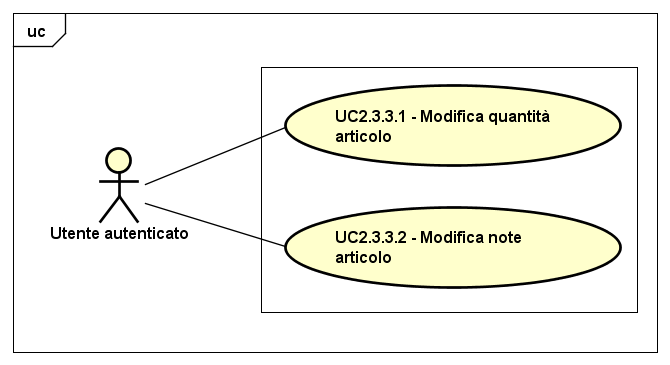
\includegraphics[width=\columnwidth]{usecase/dettaglioModifica} 
    \caption{\textit{Use Case} - UC2.3.3: Modifica articolo}
\end{figure}

\begin{itemize}
	\item \textbf{Attore}: Utente autenticato;
	\item \textbf{Descrizione}: L'attore può modificare un articolo in carrello;
	\item \textbf{Pre-condizioni}: L'attore ha avviato l'applicazione, è riconosciuto dal sistema e ha richiesto di modificare un articolo in carrello;
	\item \textbf{Post-condizioni}: L'attore ha modificato l'articolo in carrello;
	\item \textbf{Scenario principale}:
		\begin{enumerate}
			\item UC2.3.3.1 - Modifica quantità articolo;
			\item UC2.3.3.2 - Modifica note articolo.
		\end{enumerate}
\end{itemize}

\subsection{UC2.3.3.1 - Modifica quantità articolo}

\begin{itemize}
	\item \textbf{Attore}: Utente autenticato;
	\item \textbf{Descrizione}: L'attore può modificare la quantità dell'articolo selezionato;
	\item \textbf{Pre-condizioni}: L'attore ha avviato l'applicazione, è riconosciuto dal sistema, ha richiesto di modificare un articolo in carrello e il sistema permette la modifica della quantità dell'articolo selezionato;
	\item \textbf{Post-condizioni}: L'attore ha modificato la quantità dell'articolo selezionato;
	\item \textbf{Scenario principale}: L'attore modifica la quantità dell'articolo selezionato tramite una \textit{text box}.
\end{itemize}

\subsection{UC2.3.3.2 - Modifica note articolo}

\begin{itemize}
	\item \textbf{Attore}: Utente autenticato;
	\item \textbf{Descrizione}: L'attore può modificare le note dell'articolo selezionato;
	\item \textbf{Pre-condizioni}: L'attore ha avviato l'applicazione, è riconosciuto dal sistema, ha richiesto di modificare un articolo in carrello e il sistema permette la modifica della note dell'articolo selezionato;
	\item \textbf{Post-condizioni}: L'attore ha modificato le note dell'articolo selezionato;
	\item \textbf{Scenario principale}: L'attore modifica le note dell'articolo selezionato tramite una \textit{text box}.
\end{itemize}

\subsection{UC2.3.4 - Visualizzazione errore di modifica articolo}

\begin{itemize}
	\item \textbf{Attore}: Utente autenticato;
	\item \textbf{Descrizione}: L'attore inserisce una quantità non permessa per l'articolo selezionato;
	\item \textbf{Pre-condizioni}: L'attore ha avviato l'applicazione, è riconosciuto dal sistema, ha richiesto di modificare un articolo in carrello e ha inserito una quantità non permessa per l'articolo selezionato;
	\item \textbf{Post-condizioni}: L'attore ha visualizzato un messaggio d'errore relativo all'impossibilità di modificare l'articolo selezionato;
	\item \textbf{Scenario principale}: L'attore visualizza un messaggio d'errore relativo all'impossibilità di modificare l'articolo selezionato.
\end{itemize}

\subsection{UC2.3.5 - Selezione singolo articolo}

\begin{itemize}
	\item \textbf{Attore}: Utente autenticato;
	\item \textbf{Descrizione}: L'attore può selezionare un articolo non ancora selezionato in carrello;
	\item \textbf{Pre-condizioni}: L'attore ha avviato l'applicazione, è riconosciuto dal sistema e ha richiesto di selezionare un articolo non ancora selezionato in carrello;
	\item \textbf{Post-condizioni}: L'attore ha selezionato l'articolo in carrello;
	\item \textbf{Scenario principale}: L'attore seleziona l'articolo in carrello tramite una \textit{checkbox}.
\end{itemize}

\subsection{UC2.3.6 - Deselezione singolo articolo}

\begin{itemize}
	\item \textbf{Attore}: Utente autenticato;
	\item \textbf{Descrizione}: L'attore può deselezionare un articolo selezionato in carrello;
	\item \textbf{Pre-condizioni}: L'attore ha avviato l'applicazione, è riconosciuto dal sistema e ha richiesto di deselezionare un articolo selezionato in carrello;
	\item \textbf{Post-condizioni}: L'attore ha deselezionato l'articolo in carrello;
	\item \textbf{Scenario principale}: L'attore deseleziona l'articolo in carrello tramite una \textit{checkbox}.
\end{itemize}

\subsection{UC2.3.7 - Selezione totale di articoli}

\begin{itemize}
	\item \textbf{Attore}: Utente autenticato;
	\item \textbf{Descrizione}: L'attore può selezionare tutti gli articoli in carrello non ancora selezionati;
	\item \textbf{Pre-condizioni}: L'attore ha avviato l'applicazione, è riconosciuto dal sistema e ha richiesto di selezionare tutti gli articoli in carrello non ancora selezionati;
	\item \textbf{Post-condizioni}: L'attore ha selezionato tutti gli articoli in carrello non ancora selezionati;
	\item \textbf{Scenario principale}: L'attore seleziona tutti gli articoli in carrello non ancora selezionati premendo su un bottone.
\end{itemize}

\subsection{UC2.3.8 - Deselezione totale di articoli}

\begin{itemize}
	\item \textbf{Attore}: Utente autenticato;
	\item \textbf{Descrizione}: L'attore può deselezionare tutti gli articoli in carrello;
	\item \textbf{Pre-condizioni}: L'attore ha avviato l'applicazione, è riconosciuto dal sistema e ha richiesto di deselezionare tutti gli articoli selezionati in carrello;
	\item \textbf{Post-condizioni}: L'attore ha deselezionato tutti gli articoli selezionati in carrello;
	\item \textbf{Scenario principale}: L'attore deseleziona tutti gli articoli selezionati in carrello premendo su un bottone.
\end{itemize}

\subsection{UC2.3.9 - Rimozione articoli selezionati}

\begin{itemize}
	\item \textbf{Attore}: Utente autenticato;
	\item \textbf{Descrizione}: L'attore può rimuovere dal carrello gli articoli selezionati;
	\item \textbf{Pre-condizioni}: L'attore ha avviato l'applicazione, è riconosciuto dal sistema e ha richiesto di rimuovere dal carrello gli articoli selezionati;
	\item \textbf{Post-condizioni}: L'attore ha rimosso dal carrello gli articoli selezionati;
	\item \textbf{Scenario principale}: L'attore rimuove dal carrello gli articoli selezionati premendo su un bottone.
\end{itemize}

\newpage

\subsection{UC2.3.10 - Invio ordine}

\begin{figure}[!h] 
    \centering 
    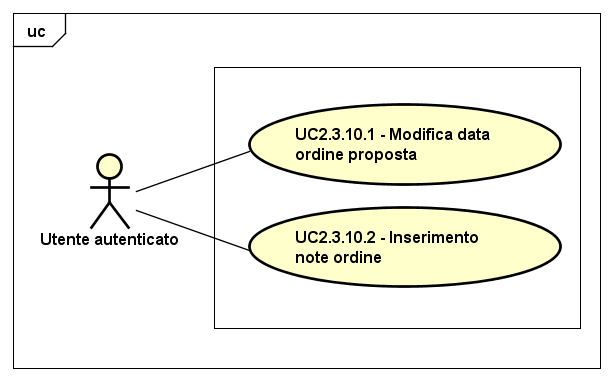
\includegraphics[width=\columnwidth]{usecase/dettaglioInvioOrdine} 
    \caption{\textit{Use Case} - UC2.3.10: Invio ordine}
\end{figure}

\begin{itemize}
	\item \textbf{Attore}: Utente autenticato;
	\item \textbf{Descrizione}: L'attore può inviare un ordine composto dagli articoli selezionati in carrello;
	\item \textbf{Pre-condizioni}: L'attore ha avviato l'applicazione, è riconosciuto dal sistema e ha richiesto di inviare un ordine composto dagli articoli selezionati in carrello;
	\item \textbf{Post-condizioni}: L'attore ha inviato un ordine composto dagli articoli selezionati in carrello;
	\item \textbf{Scenario principale}:
		\begin{enumerate}
			\item UC2.3.10.1 - Modifica data ordine proposta;
			\item UC2.3.10.2 - Inserimento note ordine.
		\end{enumerate}
\end{itemize}

\subsection{UC2.3.10.1 - Modifica data ordine proposta}

\begin{itemize}
	\item \textbf{Attore}: Utente autenticato;
	\item \textbf{Descrizione}: L'attore può modificare la data d'ordine proposta;
	\item \textbf{Pre-condizioni}: L'attore ha avviato l'applicazione, è riconosciuto dal sistema, ha richiesto di inviare un ordine e il sistema permette la modifica della data d'ordine proposta;
	\item \textbf{Post-condizioni}: L'attore ha modificato la data d'ordine proposta;
	\item \textbf{Scenario principale}: L'attore modifica la data d'ordine proposta tramite una \textit{text box}.
\end{itemize}

\subsection{UC2.3.10.2 - Inserimento note ordine}

\begin{itemize}
	\item \textbf{Attore}: Utente autenticato;
	\item \textbf{Descrizione}: L'attore può inserire delle note per l'ordine;
	\item \textbf{Pre-condizioni}: L'attore ha avviato l'applicazione, è riconosciuto dal sistema, ha richiesto di inviare un ordine e il sistema permette l'inserimento di note per l'ordine;
	\item \textbf{Post-condizioni}: L'attore ha inserito delle note per l'ordine;
	\item \textbf{Scenario principale}: L'attore inserisce delle note per l'ordine tramite una \textit{text area}.
\end{itemize}

\subsection{UC2.3.11 - Visualizzazione errore di mancata selezione di articoli}

\begin{itemize}
	\item \textbf{Attore}: Utente autenticato;
	\item \textbf{Descrizione}: L'attore preme sul bottone per la rimozione degli articoli o per l'invio di un ordine, senza aver selezionato degli articoli in carrello;
	\item \textbf{Pre-condizioni}: L'attore ha avviato l'applicazione, è riconosciuto dal sistema, ha richiesto di rimuovere degli articoli dal carrello o di inviare un ordine, senza aver effettivamente selezionato degli articoli in carrello;
	\item \textbf{Post-condizioni}: L'attore ha visualizzato un messaggio d'errore relativo all'impossibilità di rimuovere gli articoli selezionati o di inviare un ordine composto dagli articoli selezionati;
	\item \textbf{Scenario principale}: L'attore visualizza un messaggio d'errore relativo all'impossibilità di rimuovere gli articoli selezionati o di inviare un ordine composto dagli articoli selezionati.
\end{itemize}

\newpage

\section{Requisiti}

In questa sezione vengono presentati i requisiti della piattaforma \textit{moviORDER}, dedotti dai diagrammi dei casi d'uso, dal capitolato fornito da \visione{} e da raffinamenti di questo, ottenuti in seguito a brevi interazioni avvenute con il \textit{tutor} aziendale. I requisiti sono stati classificati dallo stagista in base alla loro tipologia ed importanza strategica. Sono stati individuati:
\begin{enumerate}
	\item \textbf{requisiti funzionali}: descrivono funzionalità del sistema;
	\item \textbf{requisiti qualitativi}: descrivono qualità del prodotto finale;
	\item \textbf{requisiti di vincolo}: descrivono vincoli imposti dal \textit{tutor} aziendale o dal dominio del problema.
\end{enumerate}

L'importanza strategica dei requisiti individuati è stata negoziata con il \textit{tutor} aziendale e si è deciso che ciascun requisito deve appartenere ad una delle seguenti categorie:
\begin{itemize}
	\item \textbf{obbligatorio}: non più negoziabile e irrinunciabile per il \textit{tutor} aziendale;
	\item \textbf{desiderabile}: rappresenta un valore aggiunto d'interesse riconosciuto da parte del \textit{tutor} aziendale;
	\item \textbf{facoltativo}: relativamente utile per gli scopi dell'applicazione.
\end{itemize}

Nelle seguenti sezioni vengono dettagliati i requisiti di \textit{moviORDER}. In ogni sezione è presente una tabella contenente per ogni requisito:
\begin{itemize}
	\item \textbf{codice identificativo}: codice che identifica univocamente il requisito, utile a fini di \glossaryItem{tracciabilità};
	\item \textbf{descrizione}: breve descrizione testuale del requisito;
	\item \textbf{fonte}: fonte da cui è stato dedotto il requisito, utile a fini di tracciabilità. La fonte di un requisito può essere:
		\begin{itemize}
			\item \textbf{caso d'uso}: se il requisito è stato dedotto da un caso d'uso specifico;
			\item \textbf{capitolato}: se il requisito è stato dedotto dal capitolato d'appalto;
			\item \textbf{stagista}: se il requisito è stato introdotto dallo stagista durante il periodo di \textit{stage};
			\item \textbf{\textit{tutor}}: se il requisito è stato introdotto dal \textit{tutor} aziendale durante il periodo di \textit{stage}.
		\end{itemize}
\end{itemize}

\newpage

\subsection{Requisiti funzionali}

Per facilitare la lettura della tabella il codice dei requisiti macroscopici viene evidenziato con una dicitura in grassetto. Per requisiti macroscopici si intendono i requisiti che presentano sotto-requisiti.

{\renewcommand{\arraystretch}{2}
\begin{center}
\begin{longtable}{ | >{\centering\arraybackslash}p{2.5cm} | >{\arraybackslash}p{7.1cm} | >{\centering\arraybackslash}p{2cm} | }
        
\hline
\textbf{Id Requisito} & \textbf{Descrizione} & \textbf{Fonti} \\ \hline
\endhead
RFO1 & Se l'applicazione viene lanciata in assenza di connettività, deve essere visualizzato un messaggio d'errore di connettività assente e deve essere chiusa & Stagista \\ \hline
\textbf{RFO2} & L'utente non autenticato deve poter accedere all'applicazione & Capitolato UC1.1 \\ \hline
RFO2.1 & Per accedere, l'utente non autenticato deve poter inserire una \textit{username} & Capitolato UC1.1.1 \\ \hline
RFO2.2 & Per accedere, l'utente non autenticato deve poter inserire una \textit{password} & Capitolato UC1.1.2 \\ \hline
RFO2.3 & L'utente non autenticato deve poter tentare l'accesso premendo su un bottone di \textit{login} & Capitolato\\ \hline
RFO2.4 & Se l'utente non autenticato inserisce una \textit{username} non esistente e preme sul bottone di \textit{login}, deve essere visualizzato un messaggio d'errore di \textit{username} inesistente & UC1.2 \\ \hline
RFO2.5 & Se l'utente non autenticato inserisce una \textit{password} non corrispondente alla \textit{username} inserita e preme sul bottone di \textit{login}, deve essere visualizzato un messaggio d'errore di \textit{password} errata & UC1.2 \\ \hline
RFO2.6 & Se l'utente non autenticato preme sul bottone di \textit{login} senza aver inserito le credenziali di accesso, deve essere visualizzato un messaggio che inviti l'utente ad inserire delle credenziali & UC1.2 \\ \hline
RFO2.7 & Se in fase di \textit{login} il \textit{server} non risponde, deve essere visualizzato un messaggio d'errore che notifichi l'utente che il \textit{server} è \textit{down} & Stagista \\ \hline
\textbf{RFO3} & Se l'utente non autenticato riesce ad accedere al sistema, deve essere visualizzata la \textit{home page} dell'applicazione & Capitolato \\ \hline
RFO3.1 & L'utente autenticato deve visualizzare sulla \textit{home page} la propria ragione sociale & Capitolato \\ \hline
RFO3.2 & L'utente autenticato deve poter visualizzare sulla \textit{home page} il \textit{tutorial} dell'applicazione & UC2.2 \\ \hline
RFO3.3 & L'utente autenticato deve poter effettuare il \textit{logout} dall'applicazione premendo su un bottone & UC2.1 \\ \hline
\textbf{RFO3.4} & L'utente autenticato deve poter visualizzare sulla \textit{home page} i propri articoli nel carrello & Capitolato \\ \hline
RFO3.4.1 & Se l'utente autenticato non presenta articoli in carrello, deve essere visualizzato un messaggio che notifichi l'utente che il carrello è vuoto & Stagista \\ \hline
RFO3.4.2 & La visualizzazione di un articolo in carrello deve comprendere una \textit{checkbox} per la selezione dell'articolo & Capitolato \\ \hline
RFO3.4.3 & La visualizzazione di un articolo in carrello deve comprendere la quantità dell'articolo & Capitolato \\ \hline
RFO3.4.4 & La visualizzazione di un articolo in carrello deve comprendere il codice dell'articolo & Capitolato \\ \hline
RFO3.4.5 & La visualizzazione di un articolo in carrello deve comprendere la descrizione dell'articolo & Capitolato \\ \hline
\textbf{RFO3.5} & L'utente autenticato deve poter aggiungere un nuovo articolo al carrello & Capitolato UC2.3.1 \\ \hline
RFO3.5.1 & Per aggiungere un nuovo articolo al carrello, l'utente autenticato deve inserire un codice articolo & Capitolato UC2.3.1.1 \\ \hline
RFO3.5.2 & L'utente autenticato deve poter decidere se inserire il codice articolo con la scansione di un codice a barre o manualmente & Capitolato UC2.3.1.1 \\ \hline
\textbf{RFO3.5.3} & Se l'utente autenticato decide di inserire il codice articolo con la scansione di un codice a barre, l'applicazione deve accedere alla fotocamera e permettere la cattura del codice a barre & Capitolato UC2.3.1.3 \\ \hline
RFO3.5.3.1 & L'applicazione deve permettere la cattura di un codice a barre di tipo \textit{EAN13} & Capitolato \\ \hline
RFO3.5.3.2 & L'applicazione deve permettere la cattura di un codice a barre di tipo \textit{EAN8} & Capitolato \\ \hline
RFO3.5.3.3 & L'applicazione deve permettere la cattura di un codice a barre di tipo \textit{CODE39} & Capitolato \\ \hline
RFO3.5.3.4 & L'applicazione deve permettere la cattura di un codice a barre di tipo \textit{UPC} & Capitolato \\ \hline
RFO3.5.3.5 & L'applicazione deve permettere la cattura di un codice a barre di tipo \textit{QR} & Capitolato \\ \hline
RFO3.5.3.6 & L'utente autenticato deve poter annullare la scansione del codice a barre con il tasto indietro del sistema operativo & Stagista \\ \hline
RFO3.5.3.7 & Se l'utente autenticato annulla la scansione del codice a barre, deve essere visualizzato un messaggio di annullamento della scansione da parte dell'utente & UC2.3.2 \\ \hline
RFO3.5.3.8 & Se la scansione del codice a barre fallisce, la fotocamera deve essere chiusa e deve essere visualizzato un messaggio d'errore di scansione fallita & UC2.3.2 \\ \hline
RFO3.5.3.9 & Se la scansione del codice a barre va a buon fine ma il codice ottenuto non corrisponde ad un articolo venduto dall'azienda, deve essere visualizzato un messaggio d'errore che notifichi l'utente autenticato del problema & UC2.3.2 \\ \hline
RFO3.5.3.10 & Se la scansione del codice a barre va a buon fine e il codice ottenuto corrisponde ad un articolo venduto dall'azienda ma l'articolo è già presente in carrello, deve essere visualizzato un messaggio che inviti l'utente autenticato a cambiare la quantità dell'articolo in carrello & UC2.3.2 \\ \hline
RFO3.5.3.11 & Se la scansione del codice a barre va a buon fine e il codice ottenuto corrisponde ad un articolo venduto dall'azienda, deve essere visualizzata la pagina per l'aggiunta dell'articolo & Capitolato \\ \hline
\textbf{RFO3.5.4} & Se l'utente autenticato decide di inserire il codice articolo manualmente, deve essere visualizzata una \textit{text box} per l'inserimento del codice & Capitolato UC2.3.1.2 \\ \hline
RFO3.5.4.1 & Se l'utente autenticato inserisce un codice che non corrisponde ad un articolo venduto dall'azienda, deve essere visualizzato un messaggio d'errore che notifichi l'utente del problema & UC2.3.2 \\ \hline
RFO3.5.4.2 & Se l'utente autenticato inserisce un codice che corrisponde ad un articolo venduto dall'azienda ma l'articolo è già presente in carrello, deve essere visualizzato un messaggio che inviti l'utente a cambiare la quantità dell'articolo in carrello & UC2.3.2 \\ \hline
RFO3.5.4.3 & Se l'utente autenticato inserisce un codice che corrisponde ad un articolo venduto dall'azienda, deve essere visualizzata la pagina per l'aggiunta dell'articolo & Capitolato \\ \hline
RFO3.5.5 & Nella pagina per l'aggiunta dell'articolo, l'utente autenticato deve poter visualizzare il codice dell'articolo & Capitolato \\ \hline
RFO3.5.6 & Nella pagina per l'aggiunta dell'articolo, l'utente autenticato deve poter visualizzare la descrizione dell'articolo & Capitolato \\ \hline
RFO3.5.7 & Nella pagina per l'aggiunta dell'articolo, l'utente autenticato deve poter visualizzare le informazioni dell'articolo & Capitolato \\ \hline
RFO3.5.8 & La pagina per l'aggiunta dell'articolo deve proporre all'utente autenticato una quantità minima per l'articolo da ordinare & Capitolato \\ \hline
RFO3.5.9 & Nella pagina per l'aggiunta dell'articolo, l'utente autenticato deve poter inserire una quantità per l'articolo da ordinare & Capitolato UC2.3.1.4 \\ \hline
RFO3.5.10 & Nella pagina per l'aggiunta dell'articolo, l'utente autenticato deve poter inserire delle note per l'articolo da ordine & Capitolato UC2.3.1.5\\ \hline
RFO3.5.11 & Nella pagina per l'aggiunta dell'articolo, l'utente autenticato deve poter annullare l'inserimento dell'articolo & Capitolato \\ \hline
RFO3.5.12 & Nella pagina per l'aggiunta dell'articolo, l'utente autenticato deve poter confermare l'inserimento dell'articolo & Capitolato \\ \hline
RFO3.5.13 & Se l'utente autenticato conferma l'inserimento dell'articolo e ha inserito una quantità errata (troppo bassa, troppo alta o che non soddisfa uno step impostato dall'azienda), deve essere visualizzato un messaggio d'errore di errata quantità inserita & UC2.3.2 \\ \hline
RFO3.5.14 & Se l'utente autenticato conferma l'inserimento dell'articolo e i dati inseriti sono corretti, deve essere visualizzata la \textit{home page} dell'applicazione e il nuovo articolo deve essere presente in carrello & Capitolato \\ \hline
RFO3.5.15 & Se l'utente autenticato annulla l'inserimento dell'articolo, deve essere visualizzata la \textit{home page} dell'applicazione e il carrello non deve aver subito cambiamenti & Capitolato \\ \hline
RFO3.5.16 & Se viene persa la connettività nella pagina per l'aggiunta dell'articolo, deve essere visualizzato un messaggio che inviti l'utente a chiudere l'applicazione per connettività assente & Stagista \\ \hline
RFO3.6 & L'utente autenticato deve poter selezionare un articolo in carrello premendo sulla relativa \textit{checkbox} & Capitolato UC2.3.5\\ \hline
RFO3.7 & L'utente autenticato deve poter deselezionare un articolo selezionato in carrello premendo sulla relativa \textit{checkbox} & Capitolato UC2.3.6 \\ \hline
RFO3.8 & L'utente autenticato deve poter selezionare tutti gli articoli in carrello premendo su un bottone ``seleziona/deseleziona tutti'' presente sulla \textit{home page} & Capitolato UC2.3.7\\ \hline
RFO3.9 & L'utente autenticato deve poter deselezionare tutti gli articoli selezionati in carrello premendo su un bottone di ``seleziona/deseleziona tutti'' presente sulla \textit{home page} & Capitolato UC2.3.8 \\ \hline
\textbf{RFO3.10} & L'utente autenticato deve poter modificare un articolo in carrello premendo sopra la visualizzazione dell'articolo sul carrello & Capitolato UC2.3.3\\ \hline
RFO3.10.1 & Se l'utente autenticato preme sulla visualizzazione di un articolo in carrello, deve essere richiesta la conferma di modifica tramite la visualizzazione di un \glossaryItem{dialog} & Stagista \\ \hline
RFO3.10.2 & Se l'utente autenticato accetta di modificare l'articolo sul \textit{dialog} di conferma, deve essere aperta la pagina la modifica dell'articolo & Stagista \\ \hline
RFO3.10.3 & Se l'utente autenticato rifiuta di modificare l'articolo sul \textit{dialog} di conferma, deve essere visualizzata la \textit{home page} senza cambiamenti sugli articoli in carrello & Stagista \\ \hline
RFO3.10.4 & Nella pagina per la modifica dell'articolo, l'utente autenticato deve poter visualizzare il codice dell'articolo selezionato & Capitolato \\ \hline
RFO3.10.5 & Nella pagina per la modifica dell'articolo, l'utente autenticato deve poter visualizzare la descrizione dell'articolo selezionato & Capitolato \\ \hline
RFO3.10.6 & Nella pagina per la modifica dell'articolo, l'utente autenticato deve poter visualizzare le informazioni dell'articolo selezionato & Capitolato \\ \hline
RFO3.10.7 & La pagina per la modifica dell'articolo deve proporre all'utente autenticato la quantità precedentemente inserita per l'articolo selezionato & Capitolato \\ \hline
RFO3.10.8 & Nella pagina per la modifica dell'articolo, l'utente autenticato deve poter cambiare la quantità per l'articolo selezionato & Capitolato UC2.3.3.1 \\ \hline
RFO3.10.9 & La pagina per la modifica dell'articolo deve proporre all'utente autenticato le note precedentemente inserite per l'articolo selezionato & Capitolato \\ \hline
RFO3.10.10 & Nella pagina per la modifica dell'articolo, l'utente autenticato deve poter modificare le note per l'articolo selezionato & Capitolato UC2.3.3.1 \\ \hline
RFO3.10.11 & Nella pagina per la modifica dell'articolo, l'utente autenticato deve poter annullare la modifica dell'articolo & Capitolato \\ \hline
RFO3.10.12 & Nella pagina per la modifica dell'articolo, l'utente autenticato deve poter confermare la modifica dell'articolo & Capitolato \\ \hline
RFO3.10.13 & Se l'utente autenticato conferma la modifica dell'articolo e ha inserito una quantità errata (troppo bassa, troppo alta o che non soddisfa uno step impostato dall'azienda), deve essere visualizzato un messaggio d'errore di errata quantità inserita & UC2.3.4 \\ \hline
RFO3.10.14 & Se l'utente autenticato conferma la modifica dell'articolo e i dati modificati sono corretti, deve essere visualizzata la \textit{home page} dell'applicazione e l'articolo modificato deve essere presente in carrello con le modifiche apportate & Capitolato \\ \hline
RFO3.10.15 & Se l'utente autenticato annulla la modifica dell'articolo, deve essere visualizzata la \textit{home page} dell'applicazione e l'articolo selezionato non deve essere stato modificato & Capitolato \\ \hline
RFO3.10.16 & Se viene persa la connettività nella pagina per la modifica dell'articolo, deve essere visualizzato un messaggio che inviti l'utente a chiudere l'applicazione per connettività assente & Stagista \\ \hline
\textbf{RFO3.11} & L'utente autenticato deve poter rimuovere gli articoli selezionati sul carrello premendo su un bottone presente sulla \textit{home page} & Capitolato UC2.3.9 \\ \hline
RFO3.11.1 & Se l'utente autenticato preme sul bottone per rimuovere gli articoli senza aver selezionato alcun articolo, deve essere visualizzato un messaggio che inviti l'utente a selezionare degli articoli & UC2.3.11 \\ \hline
RFO3.11.2 & Se l'utente autenticato preme sul bottone per rimuovere gli articoli avendo selezionato degli articoli sul carrello, deve essere richiesta la conferma di eliminazione tramite la visualizzazione di un \textit{dialog} & Stagista \\ \hline
RFO3.11.3 & Se l'utente autenticato conferma l'eliminazione sul \textit{dialog} di conferma, gli articoli precedentemente selezionati devono essere rimossi dal carrello & Capitolato \\ \hline
RFO3.11.4 & Se l'utente autenticato rifiuta l'eliminazione sul \textit{dialog} di conferma, il carrello non deve subire cambiamenti & Capitolato \\ \hline
\textbf{RFO3.12} & L'utente autenticato deve poter inviare un ordine composto dagli articoli selezionati in carrello premendo su un bottone presente sulla \textit{home page} & Capitolato UC2.3.10\\ \hline
RFO3.12.1 & Se l'utente autenticato preme sul bottone per l'invio di un ordine senza aver selezionato alcun articolo, deve essere visualizzato un messaggio che inviti l'utente a selezionare degli articoli & UC2.3.11 \\ \hline
RFO3.12.2 & Se l'utente autenticato preme sul bottone per l'invio di un ordine avendo selezionato degli articoli in carrello, deve essere visualizzato il \glossaryItem{modal} per l'invio dell'ordine & Stagista \\ \hline
RFO3.12.3 & Nel \textit{modal} per l'invio dell'ordine, l'utente autenticato deve poter visualizzare il codice cliente & Capitolato \\ \hline
RFO3.12.4 & Nel \textit{modal} per l'invio dell'ordine, l'utente autenticato deve poter visualizzare la descrizione cliente & Capitolato \\ \hline
RFO3.12.5 & Nel \textit{modal} per l'invio dell'ordine, l'utente autenticato deve poter visualizzare il codice del documento da generare per l'ordine & Capitolato \\ \hline
RFO3.12.6 & Nel \textit{modal} per l'invio dell'ordine, l'utente autenticato deve poter visualizzare la descrizione del documento da generare per l'ordine & Capitolato \\ \hline
RFO3.12.7 & Il \textit{modal} per l'invio dell'ordine deve proporre all'utente autenticato una data d'ordine, precisamente quella corrente & Capitolato \\ \hline
RFO3.12.8 & Nel \textit{modal} per l'invio dell'ordine, l'utente autenticato deve poter modificare la data d'ordine proposta & Capitolato UC2.3.10.1\\ \hline
RFO3.12.9 & Nel \textit{modal} per l'invio dell'ordine, l'utente autenticato deve poter inserire delle note per l'ordine & Capitolato UC2.3.10.2\\ \hline
RFO3.12.10 & Nel \textit{modal} per l'invio dell'ordine, l'utente autenticato deve poter confermare l'invio dell'ordine & Capitolato \\ \hline
RFO3.12.11 & Nel \textit{modal} per l'invio dell'ordine, l'utente autenticato deve poter annullare l'invio dell'ordine & Capitolato \\ \hline
RFO3.12.12 & Se l'utente autenticato decide di annullare l'invio dell'ordine, il \textit{modal} per l'invio dell'ordine deve essere chiuso & Stagista \\ \hline
RFO3.12.13 & Se l'utente autenticato decide di confermare l'invio dell'ordine, deve essere richiesta la conferma di invio ordine tramite un \textit{dialog} & Stagista \\ \hline
\textbf{RFO3.12.14} & Se l'utente autenticato conferma l'invio dell'ordine nel \textit{dialog} di conferma e l'ordine è andato a buon fine, deve essere visualizzato un messaggio di ordine inviato con successo e una \textit{mail} di conferma deve essere inviata sia all'utente che all'azienda & Capitolato \\ \hline
RFO3.12.14.1 & La \textit{mail} inviata dal sistema al momento dell'invio dell'ordine deve contenere in oggetto la data di registrazione dell'ordine & Capitolato \\ \hline
RFO3.12.14.2 & La \textit{mail} inviata dal sistema al momento dell'invio dell'ordine deve contenere in oggetto il codice azienda dell'utente che ha effettuato l'ordine & Capitolato \\ \hline
RFO3.12.14.3 & La \textit{mail} inviata dal sistema al momento dell'invio dell'ordine deve contenere in oggetto la tipologia di documento generato con la registrazione dell'ordine & Capitolato \\ \hline
RFO3.12.14.4 & La \textit{mail} inviata dal sistema al momento dell'invio dell'ordine deve contenere nel corpo il codice cliente del cliente che ha effettuato l'ordine & Capitolato \\ \hline
RFO3.12.14.5 & La \textit{mail} inviata dal sistema al momento dell'invio dell'ordine deve contenere nel corpo una tabella contenente i dati degli articoli ordinati & Capitolato \\ \hline
RFO3.12.14.6 & Per ogni articolo in tabella deve essere indicata la quantità ordinata & Capitolato \\ \hline
RFO3.12.14.7 & Per ogni articolo in tabella deve essere indicato il codice & Capitolato \\ \hline
RFO3.12.14.8 & Per ogni articolo in tabella deve essere indicata la descrizione dell'articolo & Capitolato \\ \hline
RFO3.12.14.9 & La \textit{mail} inviata dal sistema al momento dell'invio dell'ordine deve contenere nel corpo l'avviso di non rispondere alla \textit{mail} & Capitolato \\ \hline
RFO3.12.15 & Se l'utente autenticato conferma l'invio dell'ordine nel \textit{dialog} di conferma e l'ordine non è andato a buon fine, deve essere visualizzato un messaggio d'errore di mancato invio dell'ordine & Capitolato \\ \hline
RFO3.12.16 & Se l'utente autenticato annulla l'invio dell'ordine nel \textit{dialog} di conferma, il \textit{dialog} di conferma deve essere chiuso & Stagista \\ \hline
RFO3.13 & Se viene persa la connettività nella \textit{home page}, deve essere visualizzato un messaggio che inviti l'utente a chiudere l'applicazione per connettività assente & Stagista \\
\hline
\caption{Tabella del tracciamento dei requisiti funzionali}
\end{longtable}
\end{center}}

\subsection{Requisiti qualitativi}

{\renewcommand{\arraystretch}{2}
\begin{center}
\begin{longtable}{ | >{\centering\arraybackslash}p{2.5cm} | >{\arraybackslash}p{7.1cm} | >{\centering\arraybackslash}p{2cm} | }
\hline
\textbf{Id Requisito} & \textbf{Descrizione} & \textbf{Fonti} \\ \hline
\endhead
RQO1 & L'applicazione deve essere fornita di manuale utente & \textit{Tutor} \\ \hline
RQD2 & L'applicazione deve essere fornita di manuale sviluppatore & \textit{Tutor} \\ \hline
\caption{Tabella del tracciamento dei requisiti qualitativi}
\end{longtable}
\end{center}}

\newpage

\subsection{Requisiti di vincolo}

{\renewcommand{\arraystretch}{2}
\begin{center}
\begin{longtable}{ | >{\centering\arraybackslash}p{2.5cm} | >{\arraybackslash}p{7.1cm} | >{\centering\arraybackslash}p{2cm} | }
\hline
\textbf{Id Requisito} & \textbf{Descrizione} & \textbf{Fonti} \\ \hline
\endhead
RVO1 & L'applicazione deve essere sviluppata con un ambiente multipiattaforma (preferibilmente \textit{PhoneGap} o \textit{Xamarin}) & Capitolato \\ \hline
RVO2 & L'applicazione deve utilizzare il \textit{database} standard di \textit{VisionENTERPRISE}, senza modifica alla sua struttura & Capitolato \\ \hline
RVO3 & L'applicazione deve interfacciarsi con la fotocamera per la lettura di codici a barre & Capitolato \\ \hline
RVO4 & L'applicazione deve funzionare completamente \textit{online}, nessun dato deve essere memorizzato in locale e nessun \textit{database} deve essere sincronizzato & Capitolato \\ \hline
RVD5 & L'applicazione deve utilizzare un \textit{database} \textit{SQL Server} lato \textit{web} & Capitolato \\ \hline
RVD6 & L'applicazione deve supportare codici a barre bidimensionali (\textit{QRcode}) & Capitolato \\ \hline
RVF7 & L'applicazione deve condividere i dati di \textit{login} con l'applicazione \textit{moviDOC} & Capitolato \\ \hline
RVF8 & L'applicazione deve avere lo stesso stile di interfaccia di \textit{moviDOC} & Capitolato \\ \hline
RVF9 & L'applicazione deve permettere la firma digitale del cliente a fine ordine & Capitolato \\ \hline
\caption{Tabella del tracciamento dei requisiti di vincolo}
\end{longtable}
\end{center}}

\newpage

\subsection{Riepilogo requisiti}

I requisiti sono di seguito raggruppati in una tabella riepilogativa, in modo da comprendere la grandezza del progetto in termini di requisiti.

{\renewcommand{\arraystretch}{2}
\begin{center}
\begin{longtable}{ | >{\arraybackslash}p{2.2cm} | >{\centering\arraybackslash}p{2.2cm} | >{\centering\arraybackslash}p{2.2cm} | >{\centering\arraybackslash}p{2.2cm} | >{\centering\arraybackslash}p{2.2cm} | }
\hline
\textbf{Tipologia} & \textbf{Obbligatorio} & \textbf{Desiderabile} & \textbf{Facoltativo} & \textbf{Totale} \\ \hline
\endhead
\textbf{Funzionale} & 102 & 0 & 0 & 102 \\ \hline
\textbf{Qualitativo} & 1 & 1 & 0 & 2 \\ \hline
\textbf{Di vincolo} & 4 & 2 & 3 & 9 \\ \hline
\textbf{Totale} & 107 & 3 & 3 & 113 \\ \hline
\caption{Riepilogo requisiti}
\end{longtable}
\end{center}}

\subsection{Validazione dei requisiti}

Al termine dell'analisi dei requisiti lo stagista ha validato i requisiti tramite delle interazioni con il \textit{tutor} aziendale. Nello specifico, ci si è assicurati che i requisiti individuati rappresentassero il sistema richiesto dal capitolato. Per la scrittura dei requisiti lo stagista ha cercato di aderire allo standard \textit{IEEE} 830-1998, il quale individua otto qualità essenziali per i requisiti:
\begin{itemize}
	\item assenza di ambiguità;
	\item correttezza;
	\item completezza;
	\item verificabilità;
	\item consistenza;
	\item modificabilità;
	\item tracciabilità;
	\item ordinamento per rilevanza.
\end{itemize}